\section{Hamming Code}
Channel coding theorem 证明了存在编码方式使得 transmit imformation at rate $R<C$, 在$n\to \infty$时 可以达到任意小的error probability $p_e^{(n)}$.

LDPC(Low Density Parity Check) code, polar code 等编码方式可以信道容量的任意接近, Hamming code 可以检验错误的位置(发生错误的数量较少时可以纠正, 稍微多一点只能发现错误无法纠正, 再多无法发现).

\textcolor{blue}{编码时涉及到的加法运算均为模2加法}.

\begin{definition}
Hamming Code. $H$为奇偶校验矩阵(parity check matrix). $H$的每一列是 $1,\ldots, 7$对应的二进制.
\end{definition}
\begin{figure}[htbp]
    \centering
    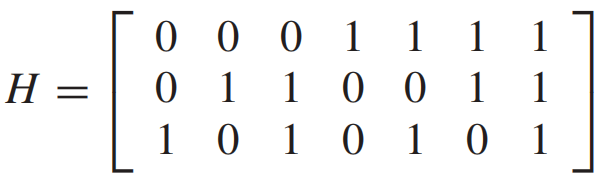
\includegraphics[width=0.5\textwidth]{./figures/chapter5/parity_check_matrix.png}
\end{figure}
例子中$H_{3\times 7}$, $\text{rank}(H)=3$, $\text{nullity}(H)=7-3=4$. 所以$H$的零空间中共有$2^{\text{nullity}(H)}=2^4=16$个向量. 如图所示:

\begin{figure}[htbp]
    \centering
    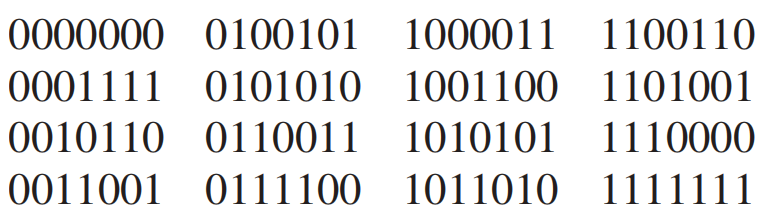
\includegraphics[width=0.5\textwidth]{./figures/chapter5/null(H).png}
\end{figure}

零空间的所有向量构成codebook $\mathcal{C}$, 且零空间是一个线性空间. Sense the sum of any two codewords is also a codeword. 将 $\mathcal{C}$中的codeword $\mathbf{c}_1,\mathbf{c}_2$看作列向量, 则 $Hc_1=0, Hc_2=0\Rightarrow H(\mathbf{c}_1+\mathbf{c}_2)=0$.

其中每一个向量的前$k$位(例子中$k=4$)位信息位 information bits, 后$n-k$位(例子中$n=7, n-k=3$)为校验位 parity check bits. 一个$(n,k)$-code 的传输速率为 $\textcolor{red}{R=\dfrac{k}{n}}$.

recall: 信道编码的目的是增加传输位数上的冗余, 以增加信息传输的可靠性. 所以我们尽可能的增强code的纠错能力.

\begin{definition}
Hamming Distance between codeword $\mathbf{a}$ and $\mathbf{b}$: 两个码字中不同的bit的个数. (Actually $\|\mathbf{a}-\mathbf{b}\|_0$).
\end{definition}
The minimum weight of a code: $\mathcal{C}$中除了全0码字外, 码字中$1$的个数的最小值. Actually, minimum weight = $d_{\min}$. \\
在$(7,3)$-code 中, 任意两个码字之间的Hamming Distance最小值$d_{\min}=3$.
\begin{figure}[htbp]
    \centering
    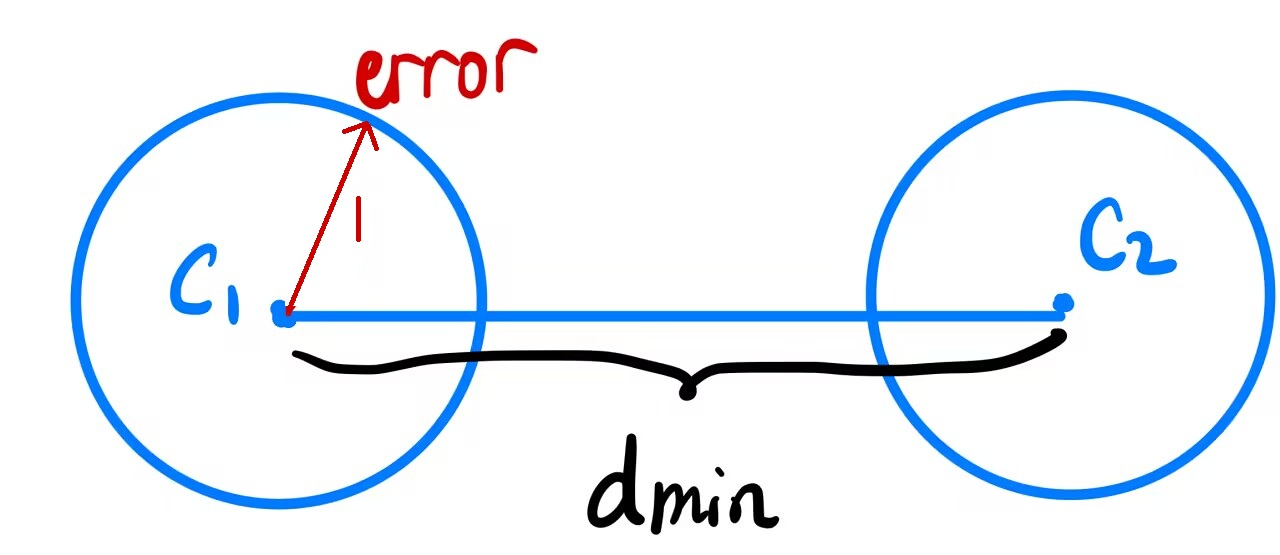
\includegraphics[width=0.5\textwidth]{./figures/chapter5/error.png}
\end{figure}

Hamming code可以纠正$\left\lfloor \dfrac{d_{\min}-1}{2} \right\rfloor$个错误, 检测到 $d_{\min}-1$个错误. \\
例如$(7,3)$-code可以纠正1个错误. 但是如果有2个错误, 则无法纠正, 只能检测. 若有$\geq 3$个错误, 则无法检测出来.

\begin{example}
若只发生一个错误: Let $\mathbf{x}$ be the input, 第$i$位发生错误, 则接收到的信号为 $\mathbf{r}=\mathbf{x}+\mathbf{e}_i$.
则
$$H\mathbf{r}=H(\mathbf{x}+\mathbf{e}_i)=H\mathbf{x}+H\mathbf{e}_i=H\mathbf{e}_i=\mathbf{h}_i$$
由于$H$矩阵第$i$列为$\mathbf{h}_i$, 转成$2$进制后即为列数本身, 则可直接找到第$i$位发生错误.
\end{example}

\begin{proposition}
Hamming code的构建: 通常若矩阵的行数为$l$, 则设列数(Hamming code的长度)为: $n=2^l-1$, 信息位数$k=\text{nullity}(H)=n-l=2^l-1-l$. 通常设$d_{\min}=3$. 即$(2^l-1,2^l-1-l,3)$-code 或写作$(2^l-1,2^l-1-l)$-code.
\end{proposition}
$$R=\dfrac{k}{n}=\dfrac{2^l-1-l}{2^l-1}$$
随着$l$的增加, $R$逐渐从小接近到$1$. \\
当 $R<C$时, 错误概率$p_e^{(n)}\to 0$. $R>C$时, 错误概率$p_e^{(n)}\not\to 0$.
\begin{example}
For a BSC using Hamming code, $C=1-H(p), R = \dfrac{k}{n} = \dfrac{2^l-1-l}{2^l-1}$, 当$p=\dfrac{1}{2}$时, $C=1-H(\dfrac{1}{2})=0, R>0$, 所以此时传输一定会出错. \\
\end{example}

可以用Venn图来理解Hamming code:
\begin{figure}[htbp]
    \centering
    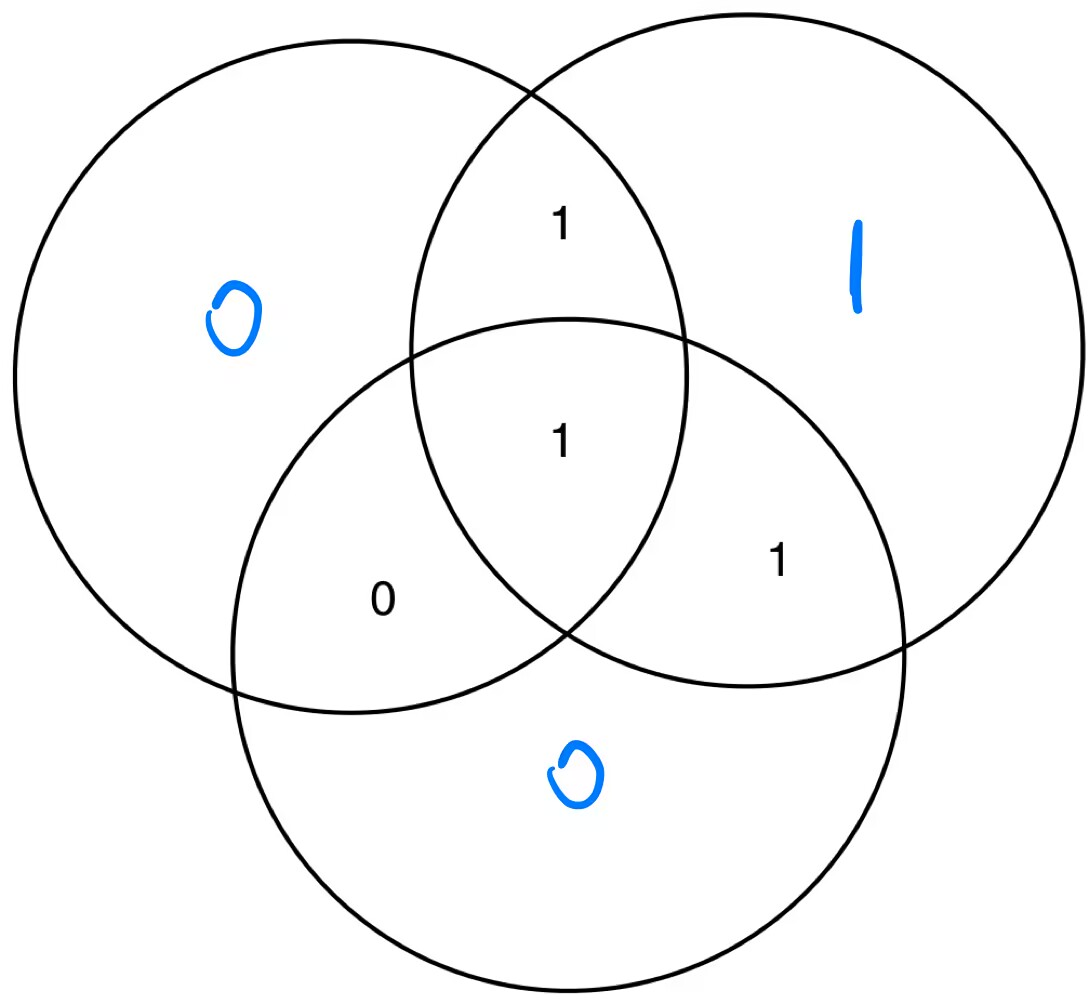
\includegraphics[width=0.5\textwidth]{./figures/chapter5/parity_check_venn.png}
\end{figure}
假设code为 1101\textcolor{blue}{001}, 中间有交集的部分放置信息位(1101), 边放置校验位\textcolor{blue}{001},其中在放置校验位时, 保证每个大圆中$1$的个数为偶数. 若无法保证, 则检测到错误. \\
纠错方式: 在Venn图中更改某一位, 使得满足要求. 或者在码本中找与当前错误的码字Hamming Distance最小的码字进行替换.